%# -*- coding: utf-8-unix -*-
%%==================================================
%% chapter01.tex for SJTU Master Thesis
%%==================================================

%\bibliographystyle{sjtu2}%[此处用于每章都生产参考文献]
\chapter{绪论}
\label{chap:intro0}

\section{自动语音识别}
\label{chap:intro0-asr}


在日常生活中,语音是人与人之间交流最主要也是最有效的方式。目前的人机交互方式主要由键盘、鼠标和触摸屏来完成,随着移动设备的不断发展,过去的人机交互方式已经不再适用。用语音来进行人机交互能极大的提高移动设备的易用性。使用语音来进行人机交互包含语音识别、语义理解、对话管理和语音合成等关键技术,而其中自动语音识别(Automatic Speech Recognition, ASR)作为整个闭环的入口无疑是最重要的一环。它的功能就是将人的语音转换为相应的文本或者指令以用于后续的处理。

\subsection{语音识别简史}
\label{chap:intro0-asr-history}


最早的语音识别系统出现在1952年的贝尔实验室~\cite{davis1952automatic},这是一个只能进行孤立的数字识别的系统。它没有使用通用计算机和任何统计机器学习的方法,只是一个精心设计的端到端的电路。现代的语音识别的基础开始于70年代,代表是隐马尔可夫(Hidden Markov Model, HMM)模型的提出~\cite{baker1975dragon, jelinek1976continuous}。在这个模型中,发声的过程被描述为一个随机生成过程,观测特征的生成过程可以被两个条件概率所描述:状态转移概率和状态输出概率。HMM被用来对发声单元进行建模,发声单元包括音素,词或者句子。在接下来的几十年里,随着混合高斯模型(Gaussian mixture model, GMM)被用于建模状态输出概率以及GMM-HMM理论的不断发展和计算资源的不断提高,语音识别得到了显著的发展。语音识别的任务也从简单的孤立词识别任务进展到大词汇连续语音识别任务。从1988年开始,美国国家标准与技术研究所(National Institute of Standards and Technology, NIST)以及美国国防部高级研究计划局(Defence Advanced Research Project Agency, DARPA)联合组织几场对连续词汇语音识别的评估。这些评估大大推进了语音识别研究的发展并为语音识别设立了若干里程碑。语音识别的词汇量从1988年资源管理任务的900个词提高到1993年华尔街日报任务的20000词,达到了真正意义上的大词汇连续语音识别。不仅仅是词汇量的增加,语音识别的任务也向着更现实的识别任务发展,比如录音环境从干净环境变成噪声环境,录音工具从专门的录音设备变成一般的电话语音。随着录音环境越来越复杂,优化的目标也从孤立的单词变为连续的词序列预测。在90年代末期,在HMM的基础上,研究者进一步提出了自适应和自适应训练技术~\cite{anastasakos1996compact,digalakis1995speaker,furui1989unsupervised,gales1998cluster,gales1998maximum,gales2001adaptive,gales2001multiple,gauvain1994maximum,kuhn1998eigenvoices,lee1996speaker,leggetter1995maximum,neumeyer1995comparative,pye1997experiments}来应对不断复杂的语音环境,以及序列鉴别性训练技术~\cite{bahl1986maximum,schluter2001comparison,chou1993minimum,goel2000minimum,juang1997minimum,povey2005discriminative,povey2001improved}来使用序列级的准则进行模型优化。这两项技术是在深度神经网络(Deep Neural Network, DNN)提出之前对GMM-HMM系统在复杂环境下提升性能最核心的技术。苹果手机的第一代Siri中使用的就是这些技术。

最早在20世纪90年代~\cite{bourlard1989continuous,bourlard1992cdnn,bourlard2012connectionist},已经有研究者提出了使用神经网络(Neural Network, NN)来对隐马尔可夫模型中的状态输出概率进行建模的方法。然而,因为那个年代计算资源与数据的匮乏,该框架并没有取得比GMM-HMM系统更好的性能。随着摩尔定律持续有效,如今的计算机的运算能力比二十年前有了巨大的飞跃。通用计算图形处理器(General Purpose Graphical Processing Units, GPGPUs)使得计算机可以更快速的进行并行计算,这使得训练更强大的模型变得可能。借助越来越先进的移动互联网和云计算,现在可以更容易的收集到足够多的训练数据。这些因素都使得深度神经网络(Deep Neural Network, DNN)在今天可以被成功地训练。DNN-HMM的提出是对GMM-HMM框架的一次变革,令语音识别的性能再次获得了巨大的提高,真正走出了实验室的研究层次~\cite{ASRBook-Yu2014,CD-DNN-HMM-dahl2012,DNN4ASR-hinton2012,qian2016very,TDNN-peddinti2015,Deepspeech2-amodei2015,LACE-yu2016,xiong2017microsoft}。谷歌、微软、苹果等国际IT巨头近年都推出了以语音识别为核心技术的商业级产品。

词错误率(Word Error Rate, WER)是衡量语音识别系统好坏的重要指标。给定正确标注和语音识别系统的解码结果,词错误率定义为两个词序列之间的编辑距离。它的数值越小越好。图~\ref{fig:WER}反映的是截止到2009年深度神经网络出来之前NIST赞助的各个语音识别任务的词错误率变迁。其中横坐标是时间,纵坐标是词错误率,每一条折线代表着一项语音识别任务。
\begin{figure}[!htp]
  \centering
    \captionstyle{\centering}
    \centering
    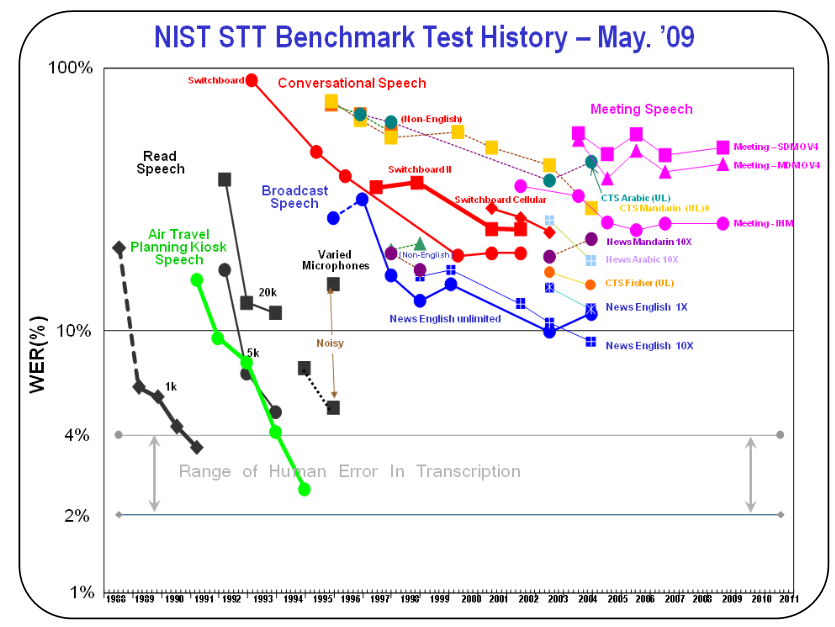
\includegraphics[width=.7\textwidth]{WER.png}
    \bicaption[fig:WER]{}{语音识别词错误率变迁图(截止2009年)}{Fig}{History of WER on several tasks (until 2009)}
\end{figure}
最早的任务是干净环境下的阅读语音识别,随着GMM-HMM模型的完善达到了和人类一样的识别率,到90年代,任务逐渐向越来越复杂的真实环境靠近。仅仅使用GMM-HMM模型,词错误依然很高。其中一个标志性的任务是Switchboard,该任务为电话语音识别。语音识别任务的两个最大难点在于,第一,语言信号是一个高度非线性的信号;第二,声学环境(说话人,噪音等)对语音信号会有很大影响。从图中可以看到,越往右边的任务场景越开放,难度也越大。在21世纪初,学者们研究了鉴别性训练和自适应方法分别用于解决这两个难题,可以看到Switchboard的词错率有了很大下降。在2010年,微软学者提出了使用深度神经网络来对语音信号进行建模,神经网络的高度非线性非常契合语音信号,Switchboard的词错误率得到了进一步下降。因为DNN-HMM框架是对GMM-HMM框架的一个变革,而序列鉴别性训练与自适应技术是与框架独立的两个技术方向。因此,它们在新框架下有了发展的新空间。最近,基于深度神经网络的序列鉴别性训练与自适应技术也成为了新时代语音识别领域最核心的研究内容。本论文主要关注于基于深度神经网络的自适应技术研究。


\subsection{语音识别架构}
\label{chap:intro0-asr-framework}


在迄今为止最为成功的基于统计的语音识别的框架中,语音识别过程可以被抽象为如下数学公式:

\begin{equation}
    \label{eq:asr}
    \mathbf{w}^* = \arg \max_{\mathbf{w} \in \mathcal{H}}P(\mathbf{w}|\mathbf{O})
\end{equation}

即在所有可能的候选假设$\mathcal{H}$中寻找拥有最大后验概率$P(\mathbf{w}|\mathbf{O})$的词序列$\mathbf{w}^*$。其中$\mathbf{w}=\left[ w_1, ..., w_n \right]$是词序列,$\mathbf{O}=\left[ \mathbf{o}_1, ..., \mathbf{o}_T \right]$是特征向量序列。

\begin{eqnarray*}
    \centering
    \mathbf{w}^* &=& \arg \max_{\mathbf{w} \in \mathcal{H}}P(\mathbf{w}|\mathbf{O}) \\
    &=& \arg \max_{\mathbf{w} \in \mathcal{H}} \frac{p(\mathbf{O}|\mathbf{w})P(\mathbf{w})}{p(\mathbf{O})} \\
    &\propto& \arg \max_{\mathbf{w} \in \mathcal{H}} p(\mathbf{O}|\mathbf{w})P(\mathbf{w}) \\
\end{eqnarray*}

直接对后验概率$P(\mathbf{w}|\mathbf{O})$建模是比较困难的,这个问题可以通过贝叶斯公式转换成条件似然$p(\mathbf{O}|\mathbf{w})$,先验$P(\mathbf{w})$和$p(\mathbf{O})$。因为边缘分布$p(\mathbf{O})$在解码过程中与假设的词无关,所以可以忽略掉。在剩下部分中,$p(\mathbf{O}|\mathbf{w})$被称为声学模型,$P(\mathbf{w})$被称为语言模型。声学模型用来建模子词单元生成特征序列的概率,语言模型描述的是局部的语法和整句话的语义信息。

\begin{figure}[!htp]
  \centering
    \captionstyle{\centering}
    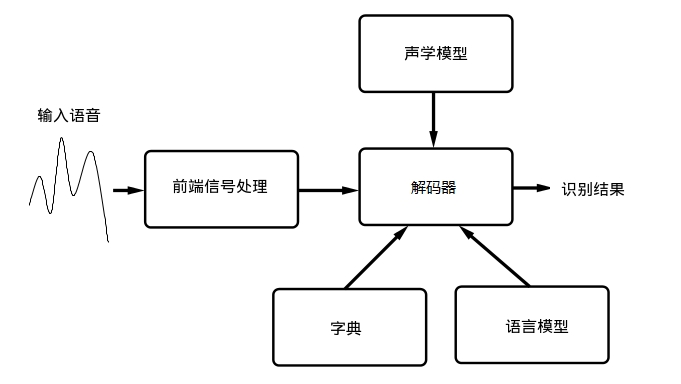
\includegraphics[width=.9\textwidth]{asr.png}
    \bicaption[fig:asr]{}{语音识别框架}{Fig}{Framework of an automatic speech recognition system}
\end{figure}

图~\ref{fig:asr}是对当前流行的语音识别系统的框架的描述,它主要由四个部分组成,包括前端信号处理、声学模型、语言模型和解码器。
\begin{itemize}
    \item 前端信号处理:原始模拟信号首先经录入器件转化为数字信号。前端信号处理部分负责从数字化后的语音中提取鲁棒的声学特征信息,主要包括多麦克风阵列降噪和提取符合人耳听觉感知的声学特征等。详细内容将在章节~\ref{sec:feat_extra}中介绍。
    \item 声学模型(Acoustic Model, AM): 声学模型是语音识别系统中最核心的模型之一。声学模型的好坏直接决定了语音识别系统的性能,也是本论文的研究重点之一。声学模型建模的是给定的词序列生成出所观测到的特征向量序列的条件概率$p(\mathbf{O}|\mathbf{w})$,目前主流的语音识别系统通常使用隐马尔可夫模型(Hidden Markov Model, HMM)来做为声学模型。在HMM中,存在一个概率分布被称为状态输出概率,这个概率可以通过使用混合高斯模型来建模,也可以通过深度神经网络来建模。使用前者的语音识别系统被称为GMM-HMM系统,使用后者的被称为DNN-HMM系统。具体内容将在章节~\ref{sec:hmm}和章节~\ref{sec:dnn_hmm}中详细介绍。
    \item 语言模型(Language Model, LM): 在过去的数十年,N元组模型(n-gram)是最主要使用的语言模型~\cite{good1953population,katz1987estimation,brown1992class}。近几年,基于深度神经网络的语言模型也开始得到发展并取得了巨大的性能提升~\cite{mikolov2010recurrent,mikolov2012statistical}。
    \item 解码器及搜索(Decoder): 解码器的功能是对声学模型计算出的声学特征概率和语言模型计算出的的语言概率进行组合来得到最大概率的词序列。目前主流的解码算法是使用基于动态规划思想的维特比算法(Viterbi Algorithm),将在~\ref{sec:decode}和~\ref{chap:intro-lvcsr}中详细介绍。
\end{itemize}

\section{自动语音识别的推理问题}
\label{chap:intro0-inf}

语音识别技术虽然相比多年以前已经有了长足的进步,但是在实际应用中还有很多
困难需要处理。其中一个最主要的难题就是语音识别的推理问题。

%TODO1: 做什么事情
语音识别既是一个模式识别问题,也包含相应的推理问题。前一个问题对各种语音、语言现象进行数学表示和描述,在基于统计学习的模式识别框架下进行建模,这决定了语音识别系统可达到的识别精度的上限。而后一个问题在给定模型的情况下,研究如何将输入语音和模型相匹配,推理得到最优识别结果,这决定了识别速度和实际可达的识别精度。
%
在语音识别的推理阶段,解码器的功能是对声学模型计算出的声学特征概率和语言模型计算出的的语言概率进行组合来得到最大概率的词序列。
%
在语音识别推理阶段,解码器是语音识别系统的核心和灵魂,所有的信息都汇集于此。它将不同来源、 不同层次、 不同性质的知识和信息关联在一起,使它们互相之间取长补短, 从而得到正确的语音识别结果。因此,如何将各种性质相异的信息有机融合是解码网络和解码算法设计中必须认真研究和解决的问题。
从解码器的作用来看,它既是语音识别研究中验证各种理论、模型、算法的
正确性的基本实验平台,也是构建实用系统的基础。因此,在解码器的设计中也
需要兼顾研究的方便与工程实际应用。

%TODO2: 有什么流派
根据上一章节的讨论,一个完整的语音识别系统包含了自底向上的五层映射关系:
语音观测到 HMM 状态、 HMM 状态到上下文相关音素、上下文相关音素到音素、
音素到词、词到句子。 语音观测无法在识别之前得知,因此语音观测到 HMM 状
态的映射需要在解码过程中动态建立,对应的声学分数也需要实时计算。
对于 HMM 状态到上下文相关音素、上下文相关音素到音素、音素到词这三层映
射关系,一旦发音字典、声学模型确定便不再改变。出于对解码效率的追求,人
们通常把它们静态地编译到解码网络中去。对于没有任何约束的大词汇连续语音识别任务而言,
词可以以任意方式组织成句, 故而从原理上讲, 词、 句间的映射关系只能在解码
过程中动态建立。 但是由于表征词与词之间关联度(概率)的 N 元文法模型在解
码前便已存在且是一个有限集合, 所以在实际中, 语言模型分数的计算却可
以用不同的方式实现。 在语音识别领域,通常根据解码器中语言模型的表示、 语
言模型状态的获取以及语言模型分数计算方法的不同把解码器分为两大流派:
\begin{itemize}
\item 动态网络解码器: 在动态网络解码器中,解码网络仅包含发音字典和声学
模型,不含有语言模型的任何信息。 语言模型状态在解码过程中随着词与词相连
成句而动态地生成、语言模型分数通过查表的方式动态获取。这类解码器的典型
代表是基于发音前缀树(Pronunciation Prefix Tree, PPT)~\cite{woodland1994large}网络的解码器。
\item 静态网络解码器: 在静态网络解码器中,解码网络不仅包含发音字典和声
学模型,也包含完整的语言模型。 语言模型状态以及状态转移以有限状态机的形
式合成进解码网络中去, 语言模型分数则作为状态转移概率存储于边上。解码时,
仅需逐边积累整条路径的状态转移概率便可获得语言模型分数。这类解码器的典
型代表是基于加权有限状态转换器(WFST)~\cite{mohri2002weighted}的解码器。
\end{itemize}

%TODO3: 近来深度学习下的发展现状和缺陷
近年来,深度学习模型被引入到语音识别的声学和语言建模当中替代传统分类器,显著改善了模式识别问题的精度。 基于深度学习的语音识别由于只是替换了分类器,语音识别的推理问题未有本质改变。
针对推理问题,基于加权有限状态机(WFST)的静态搜索空间构建技术~\cite{mohri2002weighted}和帧同步的维特比(Viterbi)网络搜索算法~\cite{forney1973viterbi}是目前性能最好的解决方案,但其仍存在一系列显著缺陷:
\begin{enumerate}
\item 该种方案基于传统的混合高斯-隐马尔科夫模型(GMM-HMM)的声学模型和N元文法(N-gram)的语言模型而提出,针对目前性能最好的基于深度学习的声学模型和语言模型的研究并不充足,如何将新型的声学和语言模型引入该框架;如何充分发挥模型性能的同时改善推理速度;如何基于多知识源给出可靠的推理置信度算法,都是有待解决的问题。
\item 该种方案基于对语音识别中各知识源(声学、语言、语义等)进行搜索空间的预先构建及整体优化,导致最终得到的搜索空间巨大,包括离线构建、在线使用、动态修改等各环节算法的计算量和内存消耗都非常大,是阻碍语音识别应用场景扩展的一个重要原因。旨在解决该问题,针对新型声学和语音模型的搜索空间整体优化研究尚不充分,而基于推理中间状态对搜索空间进行动态优化的研究几乎处于空白。
\item 目前的语音识别系统基于多知识源建模结果,对输入音频进行推理,其建模和推理过程都很复杂,且针对知识源的划分依赖很强的先验知识。海量标注或非标注语音数据的收集,以及基于并行计算的深度学习技术,使得构建直接对语音数据和文本序列进行建模的端到端模型,及其相应的识别推理算法,成为另一种可能。当前的解码框架未有这方面设计。
\end{enumerate}

因此虽然基于深度学习模型,加权有限状态机,和帧同步的维特比网络搜索算法的基于深度学习的语音识别方案已经使其发展到基本可用的程度,但其准确度依然无法满足人类之间正常交流的要求,而速度上的限制也使其无法工作在廉价和低功耗解决方案上,这些原因共同阻碍了语音识别技术的大规模商用。


\section{论文主要内容、创新点及组织结构}
\label{chap:intro0-thesis}
本论文围绕基于深度序列模型的解码搜索技术展开了一系列探索和研究,主要涉及
了基于GPU并行计算的搜索速度优化,基于标签同步解码的搜索空间优化,基于标签同步解码的统一解码框架,关键词检测的序列建模和标签同步解码等内容。

TODO 每一点做概述和总结创新点,可参考摘要和开题报告表

本文剩余章节安排如下:首先,
TODO
